\chapter{Hardware Architecture}

This chapter first provides an overview of the architecture of the
BlueBox system, followed by all the components and peripherals,
including sensors, used in the system and their significance.  The
purpose is to give a foundational understanding of the architecture
necessary for designing and architecting the firmware.

\section{System Overview}

The BlueBox prototype consists of a central board, processor, storage
element, contact and environmental microphones, accelerometer, and
the body and environment temperature sensors. The additional
electrodes attach to the central board via a DB-9 connector. The
contact microphone is attached through a standard 2.5~mm audio jack.
The body temperature sensor is attached through solder pads on the
board.  \FIG{BlueBox_Architecture} shows the overall system
architecture for BlueBox.

\begin{figure}
	\centering
	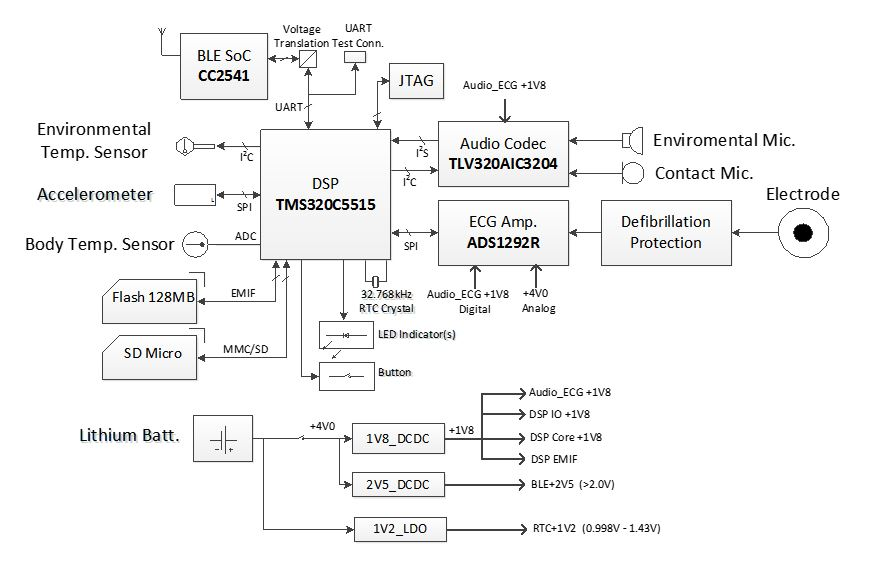
\includegraphics[scale = 0.75 ]{BlueBox_Architecture}
	\caption{BlueBox Hardware System Architecture\label{BlueBox_Architecture}}
	\label{fig:bbSysArch}
\end{figure} 


\begin{figure}
	\centering
	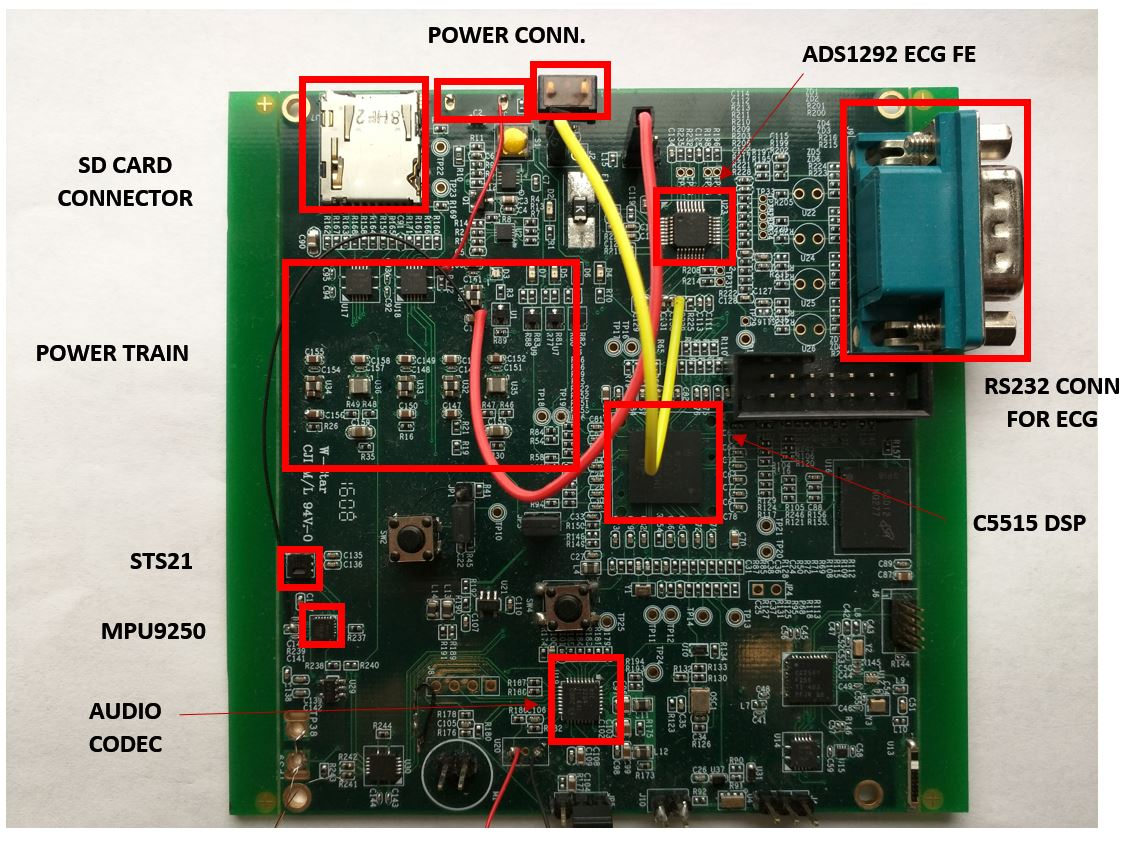
\includegraphics[scale = 0.5]{BlueBox_Hardware}
	\caption{BlueBox Prototype Hardware \label{BlueBox_Hardware}}
	\label{fig:bbHardware}
\end{figure} 

\section{Digital Signal Processor}

TMS320C5515 is a fixed-point DSP based on the TMS320C55x CPU
processor core, or C55x for short.  This DSP architecture achieves
high performance and low power through increased parallelism and
total focus on power savings. \FIG{C5515 Architecture} shows the DSP
architecture.

\begin{figure}
	\centering
	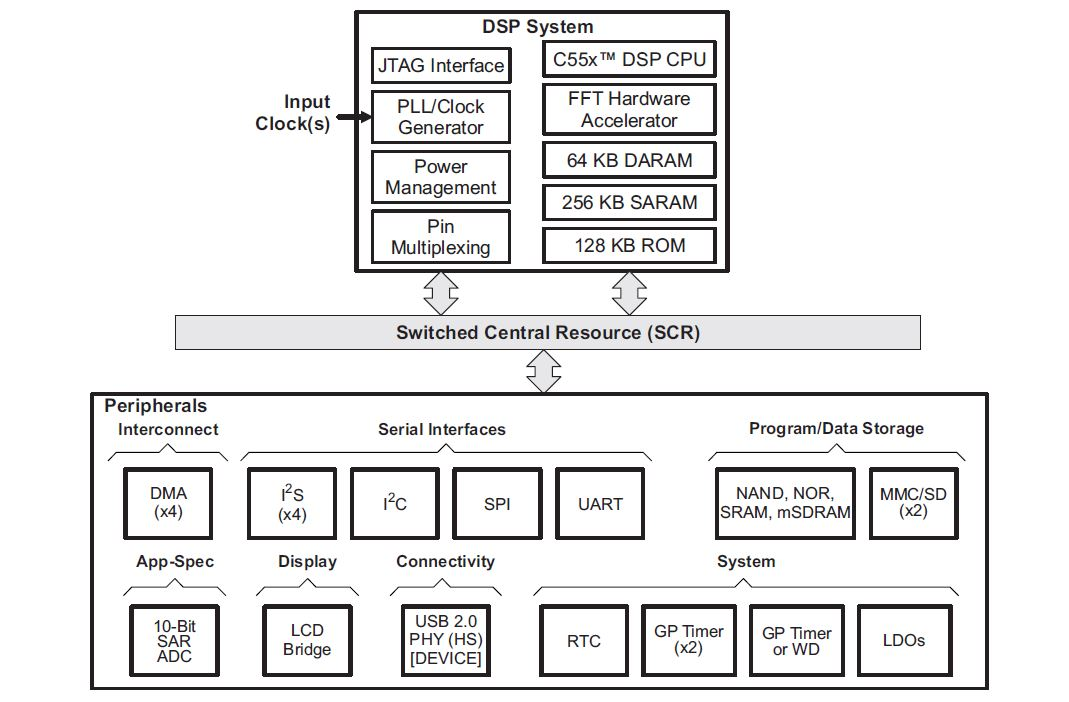
\includegraphics[scale = 0.75 ]{C5515_arch}
	\caption{DSP Architecture. \cite{tms320c5515}
	\label{C5515 Architecture}}
\end{figure} 

\subsection{Clock Frequency}

The DSP has a low power software programmable Phase Locked Loop (PLL)
clock generator that supports 60-, 75-, 100-, and 120-MHz clock rate.

\subsection{On-Chip Memory}

The DSP has 320K bytes of zero-wait-state on-chip RAM and 128K of
on-chip ROM. 

\subsection{Peripherals}

The DSP has general-purpose input and output functions along with the
10-bit Successive approximation register (SAR) Analog to Digital
converter (ADC).  Together, they provide sufficient pins for status,
interrupts, and bit I/O for LCD displays, keyboards, and media
interfaces. Serial media is supported through two Multimedia
Card/Secure Digital (MMC/SD) peripherals, four Inter-IC Sound (I2S
bus) modules, one Serial Peripheral Interface (SPI) with up to 4 chip
selects, one I$^2$C multi-master and slave interface, and a Universal
Asynchronous Receiver/Transmitter (UART) interface. 

\subsection{DMA}

The device includes four Direct Memory Access (DMA) controllers, each
with 4 channels, providing data movement for 16-independent channel
contexts without CPU intervention. Each DMA controller can perform
one 32-bit data transfer per cycle, in parallel and independent of
the CPU activity.


\subsection{Power}

Furthermore, the device includes three integrated low-dropout (LDO)
regulators (DSP LDO, ANA LDO, and USB LDO) to power different
sections of the device. The DSP LDO can provide 1.3~V or 1.05~V to
the DSP core (CVDD), selectable on-the-fly by software as long as
operating frequency ranges are observed.


\section{AIC3204 : Audio Codec}

TLV320AIC3204 (or AIC3204 for short) is an analog interface chip
(AIC) from Texas Instruments.  It is a flexible, low-power,
low-voltage stereo audio codec with programmable inputs and outputs,
PowerTune capabilities, fixed predefined and parameterizable
signal-processing blocks, integrated PLL, integrated LDOs, and
flexible digital interfaces. It has both recording and playback
capabilities. The record part of the AIC3204 covers operations from
8~kHz mono to 192~kHz stereo recording, and contains programmable
input channel configurations covering single-ended and differential
setups, as well as floating or mixing input signals. It also includes
a digitally-controlled stereo microphone preamplifier and integrated
microphone bias. It integrates A/D and D/A conversion functions and
achieved high-precision A/D and D/A converter in low cost using
$\Sigma$-$\Delta$ technology. The chip is small and compact and is
available in 5~mm $\times$ 5~mm 32-pin QFN package. 

\begin{figure}
	\centering
	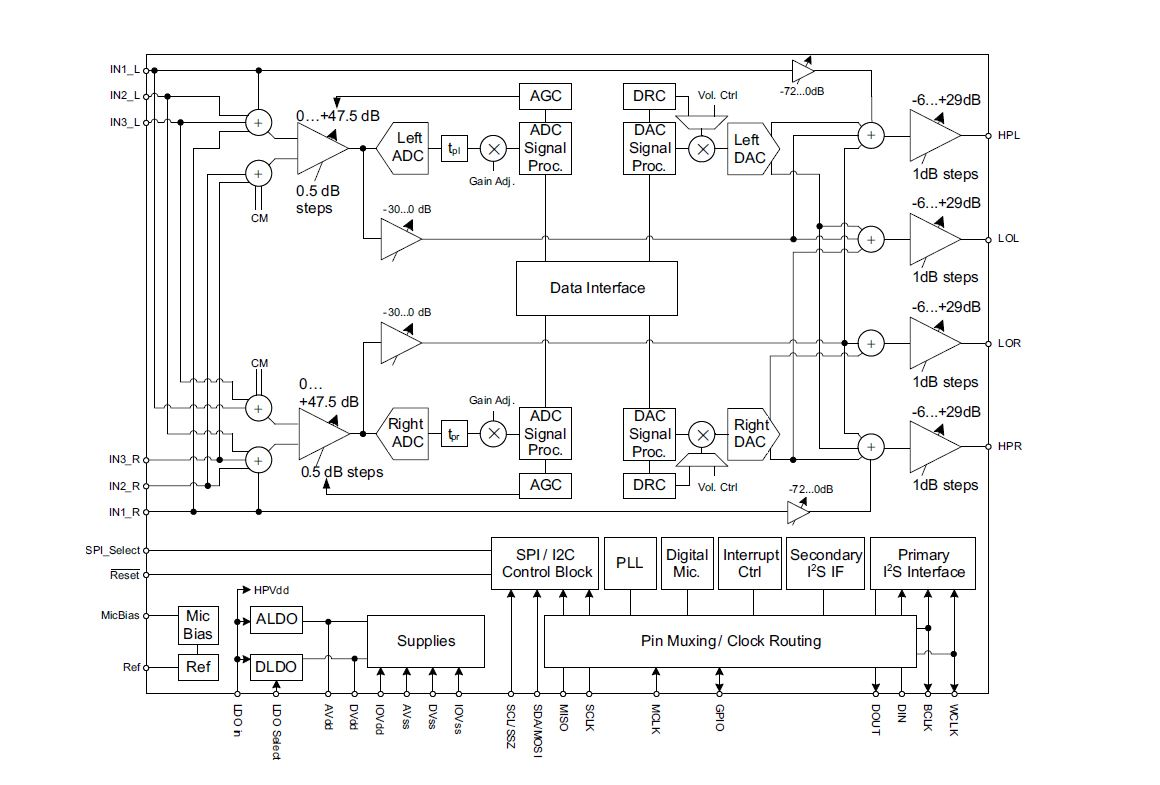
\includegraphics[scale = 0.7 ]{AIC3204}
\caption{AIC3204 Block Diagram. \cite{audiocodec}}
\label{aic3204}
\end{figure}

\FIG{aic3204} displays the audio codec's architecture. It has
capabilities of recording stereo audio signals. It has two channels
that it can record. One channel is used for respiration recording and
the other for paramedic's log recording. Each channel of the stereo
audio ADC consists of a signal-processing engine with fixed
processing blocks. The signal processing blocks available are
first-order infinite impulse response (IIR), scalable number of
bi-quad filters, variable-tap finite impulse response (FIR) filter
and automatic gain control (AGC). The choice between these processing
blocks is part of the PowerTune strategy to balance power
conservation and signal-processing flexibility. Less
signal-processing capability reduces the power consumed by the
device.

\section{ADS1292R : ECG Frontend}

ADS1292R is the ECG analog front end chip to which the electrode
output is connected to. ADS1292R is a two channel, simultaneous
sampling, 24-bit, delta-sigma ($\Delta$$\Sigma$) analog-to-digital
converters (ADCs) with a built-in programmable gain amplifier (PGA),
internal reference, and an on-board oscillator. ADS1292R incorporate
all features commonly required in portable, low-power medical
electrocardiogram (ECG), sports, and fitness applications. With high
levels of integration and exceptional performance,

\begin{cmtPai}
	(2/17) uh... ``exceptional performance'' sounds too much like
	marketing speak.  Make sure you don't copy writeup directly from
any of the product literature.
\end{cmtPai}
the ADS1292R enables the creation of scalable medical instrumentation
systems at significantly reduced size, power, and overall cost.
ADS1292R has a flexible input multiplexer per channel that can be
independently connected to the internally generated signals for test,
temperature, and lead-off detection. Additionally, any configuration
of input channels can be selected for derivation of the right leg
drive (RLD) output signal.  The ADS1292R operate at data rates from
500~SPS up to 8~kSPS. The device is packaged in a 5-mm $\times$ 5-mm,
32-pin thin quad flat pack (TQFP). Operating temperature is specified
from $-40\degC$ to $+85\degC$. ADS1292R is interfaced with the DSP
through SPI.

 \begin{figure}
 	\centering
 	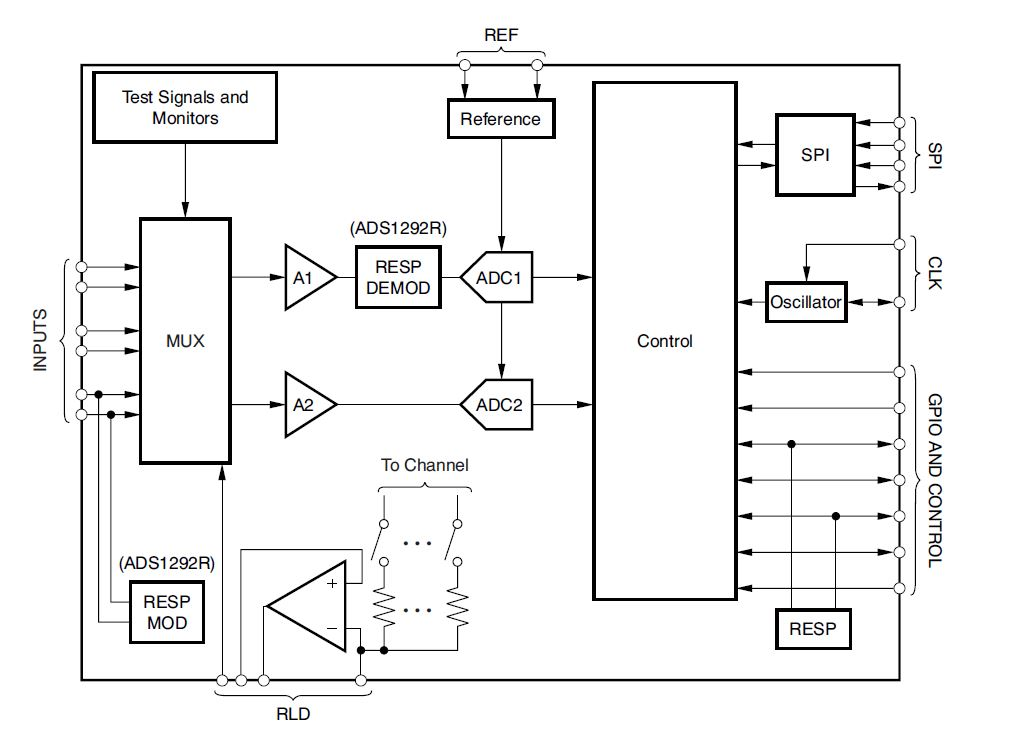
\includegraphics[scale = 0.7 ]{ADS1292R}
\caption{ADS1292R Functional Block Diagram. \cite{ads}}
\label{ADS1292R}
 \end{figure}
 
\section{MPU9250 : Accelerometer sensor}
\label{mpu9250_def}

MPU-9250 is a 9-axis motion-tracking device that combines a triaxial
gyroscope, triaxial accelerometer, and a triaxial magnetometer with a
Digital Motion Processor\textsuperscript{TM} (DMP). With its
dedicated I$^2$C sensor bus, the MPU-9250 directly provides complete
9-axis MotionFusion\textsuperscript{TM} output. MPU-9250 features
three dedicated 16-bit analog-to-digital converters (ADC) for
digitizing each of the gyroscope outputs, accelerometer outputs, and
magnetometer outputs. For precision tracking of both fast and slow
motions MPU-9250 provides a user-programmable accelerometer
full-scale range of $\pm2$~g, $\pm4$~g, $\pm8$~g, and $\pm16$~g. The
package size down to a footprint and thickness of
$3\times3\times1$~mm, to provide a very small yet high-performance
low-cost package. \FIG{mpu9250} shows the architecture of the
MPU9250.A valid accelerometer data is available 30~ms (typical) after
wakeup from sleep.

\begin{figure}
	\centering
	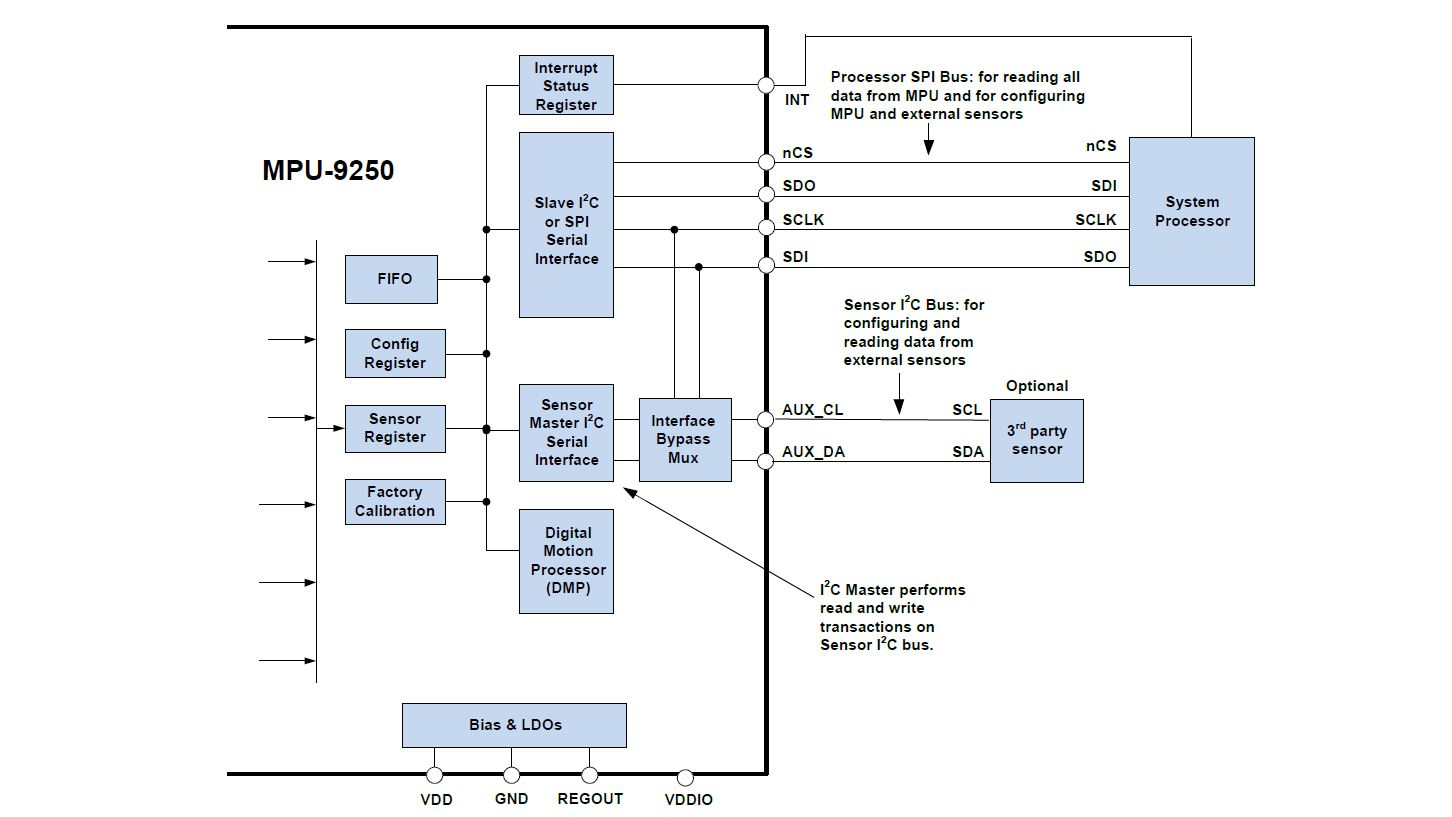
\includegraphics[scale = 0.6]{MPU9250}
\caption{MPU9250 Architecture. \cite{mpu}}
\label{mpu9250}
\end{figure}

The MPU-9250 contains a 512-byte FIFO register that is accessible via
the Serial Interface. The FIFO configuration register determines
which data is written into the FIFO. Possible choices include gyro
data, accelerometer data, temperature readings, auxiliary sensor
readings, and FSYNC input. A FIFO counter keeps track of how many
bytes of valid data are contained in the FIFO. The FIFO register
supports burst reads. The interrupt function may be used to determine
when new data is available. 

The MPU9250 has multiple user-configurable power modes. The modes of
interest are Sleep mode at 8~$\mu$A of power consumption and
Low-Power Accelerometer Mode, which consumes 450~$\mu$A. 
 
\section{Temperature sensor}

\subsection{ STS21 : Environment temperature sensor}

STS21 is a low-power, fully self-calibrated digital temperature
sensor well suited for applications with high demand on temperature
accuracy. With dedicated I$^2$C bus, it directly provides the
temperature output. The sensor comes in a package sized $3 \times
3$~mm footprint and $1.1$~mm height. The sensor is powered up to the
chosen supply voltage VDD (between 2.1~V and 3.6~V). After power-up,
the sensor needs at most 15~ms for reaching idle state, i.e., to be
ready accepting commands from the DSP. Current consumption during
start up is 350~$\mu$A maximum. Whenever the sensor is powered up,
but not performing a measurement or communicating, it is
automatically in sleep mode (idle state). STS21 measures temperature
with different resolutions ranging from 14 bits to 11 bits, where the
14-bit resolution takes 85~ms for conversion whereas a 11-bit
resolution takes somewhere between 9 and 11 ms.

\subsection{MA100: Body temperature sensor} 

MA100 is a Biomedical Chip Thermistor assemblies
\begin{cmtPai}
	(2/17/2017) how do you parse this?  I think the point is that a
	thermistor is the common type of sensor for body tempedrature
	range.  It is nonlinear in general but has very high precision (0.1
	degree?) around the body temperature range.  I know your writeup
	says it but the point does not come across as one of the key
	points.
\end{cmtPai}
that are designed for use in applications involving both intermittent
and continuous patient temperature monitoring. Although low in cost
and small in size, these are highly stable, precision thermo-chips
provide reliability, tight interchangeable tolerances, geometries,
and fast response time that are often required.
 
\section{Memory}
\label{memory}

The BlueBox system has on-chip memory and the persistent Micro-SDHC
(Secure Digital High Capacity) card storage. Because a MicroSD
card is power intensive and takes hundreds of milliseconds to write
to, the on-chip memory is used as buffer.
\begin{cmtPai}
	(2/17/2017) are you talking about memory on DSP? Or some buffer in
	the SDHC?
\end{cmtPai}
Once there is enough data in the buffer it is written to the SD card
and can be accessed by a computer.
\begin{cmtPai}
	(2/17/2017) what can be accessed by a computer?
\end{cmtPai}
All the heavy-lifting data transfers are done with the help of Direct
Memory access (DMA) peripheral interconnect to take load off the DSP.
SD card is interfaced to DSP using MMC/SD interface. The SD card used
for the application is a high capacity card that can support a
maximum clock frequency of 50~MHz. These high capacity cards are not
byte addressable. They are organized in 512-byte sector or block and
thus are block addressable. BlueBox uses Kingston 8-GB Micro SDHC
card.  The SDHC card is very power hungry. It consumes 150~mA when
operated at 50~MHz during active read/write operation and consumes
30~mA during inactive periods.

\section{Battery and Power management circuitry}

A GMB 302547 Lithium ion polymer rechargeable battery, shown in
\FIG{fig:battery}, is used to power the system. It has a
capacity of 300~mAH at 3.7~V. It is 4~cm long, 2~cm wide and 0.2~mm
\begin{cmtPai}
	(2/17/2017) are you sure 0.2 mm thick?
\end{cmtPai}
thick, and it weighs 8 grams. The battery is placed on top of the
central board housing. The central board has a battery charging
circuitry that can charge the battery completely in 2 hours. The
power management circuitry provides a power-train that feeds the
different power domain of the DSP as shown in
\FIG{BlueBox_Architecture}.

 \begin{figure}
 	\centering
 	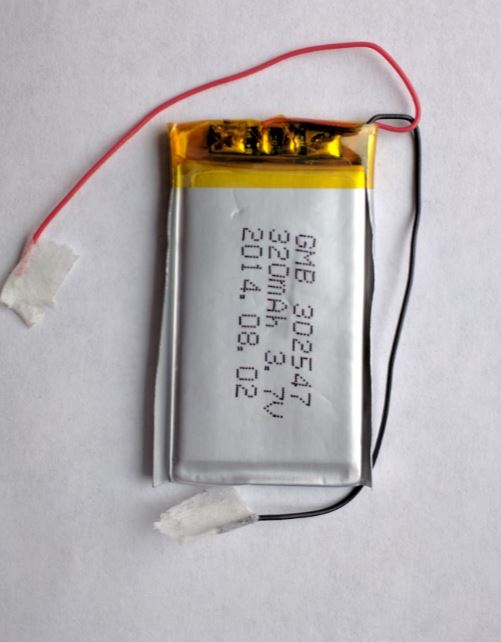
\includegraphics[scale = 0.25 ]{battery}
 	\caption{Lithium Polymer battery}\label{fig:battery}
 \end{figure}      

\nomenclature{PLL}{ Phase Locked Loop }
\nomenclature{SAR}{ Successive Approximation Register }
\nomenclature{ADC}{ Analog to Digital Converter } 
\nomenclature{I2C}{ Inter Integrated Circuit } 
\nomenclature{I2S}{ Inter-IC Sound } 
\nomenclature{SPI}{ Serial Peripheral Interface }
\nomenclature{UART}{ Universal Asynchronous Receiver/Transmitter }
\nomenclature{MMC}{ Multi Media Card }
\nomenclature{DMA}{ Direct Memory Access }
\nomenclature{LDO}{ Low DropOut }
\nomenclature{USB}{ Universal Serial Bus }
\nomenclature{RTC}{ Real-Time Clock }
\nomenclature{AIC}{ Analog Interface Chip }
\nomenclature{AGC}{ Automatic Gain Control }
\nomenclature{FIR}{ Finite Impulse  Response }
\nomenclature{IIR}{ Infinite Impulse  Response }

%%% Local Variables: ***
%%% mode: latex ***
%%% TeX-master: "thesis.tex" ***
%%% End: ***
